
\section{Проблем проналаска суме у бинарном стаблу}

\subsection{Опис проблема}
Cтабло је граф који је повезан и који нема циклуса.
Бинарно стабло је усмерено стабло у коме сваки чвор, почевши од коренског чвора, има 0, 1 или 2 деце-чворова. Дететом чвора називамо чвор на кога неки други чвор показује.
Родитељем чвора називамо чвор који на неки други чвор показује. Листом називамо чвор који има 0 деце.

\begin{figure}[H]
    \centering
    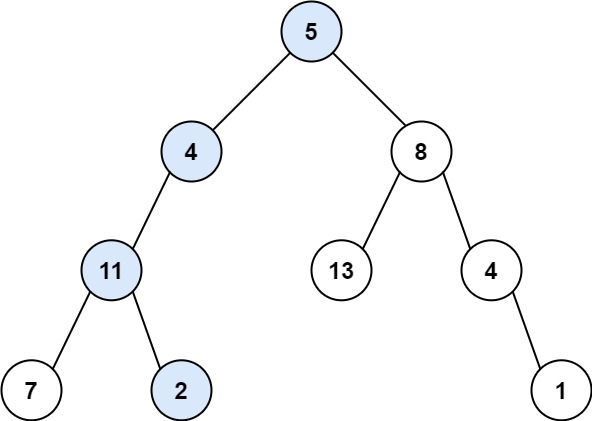
\includegraphics[scale = 0.4]{pathsum1.jpg}
    \caption{Пример постојања тражене путање за проблем проналаска суме у бинарном стаблу}
    \label{fig:primersume}
\end{figure}

У примеру \ref{fig:primersume}, плавом је приказана једна путања која даје тражену суму \textbf{22}.


\begin{table}[H]
    \centering
    \begin{tabular}{@{}c|c@{}}
        & \textbf{Улаз}           \\
        \hline
    1 & Бинарно стабло \\
    2 & Тражена сума  
    \end{tabular}
    \caption{Табела улаза за проблем проналаска суме у бинарном стаблу}
    \label{table:ulazi}
\end{table}

\begin{table}[H]
    \centering
    \begin{tabular}{@{}c|c@{}}
      & \textbf{Излаз}             \\
      \hline
    1 & Булова променљива
    \end{tabular}
    \caption{Табела излаза за проблем проналаска суме у бинарном стаблу}
    \label{table:izlazi}
\end{table}

За проблем су дата два улаза (табела \ref{table:ulazi}): стабло и тражена сума, док је тражен један излаз (табела \ref{table:izlazi}): булова променљива чија је тачност еквивалентна чињеници да је решење пронађено, односно
да за дати граф постоји путања од корена до листа која даје тражену суму.

\subsection{Секвенцијално решење проблема}

Најчешће секвенцијално решење проблема своди се на обилазак графа по дубини (енг. \textit{depth first search}, DFS).

Секвенцијално решење прво обради (по дубини) лево дете-чвор па потом десно.
Обрада појединачног чвора своди се на следећи поступак:

Постави тренутан чвор на УЛАЗ 1 (корен стабла). Постави тренутно тражену суму на УЛАЗ 2 (тражену суму).
Покрени обраду описану корацима:

\begin{enumerate}
    \item Уколико је тренутан чвор нула-чвор, врати НЕТАЧНО.
    \item Уколико тренутан чвор није нула-чвор:
    \begin{enumerate}
        \item Уколико је број придружен чвору већи од тренутно траженог збира, врати НЕТАЧНО.
        \item Уколико је број придружен чвору једнак тренутно траженом збиру и тренутни чвор је лист, врати ТАЧНО.
        \item Уколико је број придружен чвору мањи или једнак тренутно траженом збиру, умањи тренутно тражени збир за тај број. А потом:
        \begin{enumerate}
            \item Уколико обрада левог детета-чвора за тренутно тражену суму врати ТАЧНО, врати ТАЧНО.
            \item Уколико обрада десног детета-чвора за тренутно тражену суму врати ТАЧНО, врати ТАЧНО.
        \end{enumerate}
    \end{enumerate}
\end{enumerate}

У идеалном случају, решење представља путања састављена од свих левих детета-стабала. У том случају до решења се долази у асимптотском времену $О(log n)$,
где је $n$ број чворова у стаблу.
У најгорем (општем) случају ово решење има асимптотску временску сложеност извршавања $O(n)$ gde $n$ представља величину улаза tj. број чворова у графу.

Програмски код за секвенцијално решење дато је у листингу \ref{code:sekvencijalno}. Напомена: изостављен је део кода за учитавање библиотека, учитавање и креирање графа.

\begin{listing}
\inputminted{c}{kodovi/basic.c}
\caption{Имплементација секвенцијалног решења у језику \texttt{C}}
\label{code:sekvencijalno}
\end{listing}

\pagebreak
